%!TEX TS-program = xelatex

% Шаблон документа LaTeX создан в 2018 году
% Алексеем Подчезерцевым
% В качестве исходных использованы шаблоны
% 	Данилом Фёдоровых (danil@fedorovykh.ru) 
%		https://www.writelatex.com/coursera/latex/5.2.2
%	LaTeX-шаблон для русской кандидатской диссертации и её автореферата.
%		https://github.com/AndreyAkinshin/Russian-Phd-LaTeX-Dissertation-Template

\documentclass[a4paper,14pt]{article}


%%% Работа с русским языком
\usepackage[english,russian]{babel}   %% загружает пакет многоязыковой вёрстки
\usepackage{fontspec}      %% подготавливает загрузку шрифтов Open Type, True Type и др.
\defaultfontfeatures{Ligatures={TeX},Renderer=Basic}  %% свойства шрифтов по умолчанию
\setmainfont[Ligatures={TeX,Historic}]{Times New Roman} %% задаёт основной шрифт документа
\setsansfont{Comic Sans MS}                    %% задаёт шрифт без засечек
\setmonofont{Courier New}
\usepackage{indentfirst}
\frenchspacing

\renewcommand{\epsilon}{\ensuremath{\varepsilon}}
\renewcommand{\phi}{\ensuremath{\varphi}}
\renewcommand{\kappa}{\ensuremath{\varkappa}}
\renewcommand{\le}{\ensuremath{\leqslant}}
\renewcommand{\leq}{\ensuremath{\leqslant}}
\renewcommand{\ge}{\ensuremath{\geqslant}}
\renewcommand{\geq}{\ensuremath{\geqslant}}
\renewcommand{\emptyset}{\varnothing}

%%% Дополнительная работа с математикой
\usepackage{amsmath,amsfonts,amssymb,amsthm,mathtools} % AMS
\usepackage{icomma} % "Умная" запятая: $0,2$ --- число, $0, 2$ --- перечисление

%% Номера формул
%\mathtoolsset{showonlyrefs=true} % Показывать номера только у тех формул, на которые есть \eqref{} в тексте.
%\usepackage{leqno} % Нумерация формул слева	

%% Перенос знаков в формулах (по Львовскому)
\newcommand*{\hm}[1]{#1\nobreak\discretionary{}
	{\hbox{$\mathsurround=0pt #1$}}{}}

%%% Работа с картинками
\usepackage{graphicx}  % Для вставки рисунков
\graphicspath{{images/}}  % папки с картинками
\setlength\fboxsep{3pt} % Отступ рамки \fbox{} от рисунка
\setlength\fboxrule{1pt} % Толщина линий рамки \fbox{}
\usepackage{wrapfig} % Обтекание рисунков текстом

%%% Работа с таблицами
\usepackage{array,tabularx,tabulary,booktabs} % Дополнительная работа с таблицами
\usepackage{longtable}  % Длинные таблицы
\usepackage{multirow} % Слияние строк в таблице
\usepackage{float}% http://ctan.org/pkg/float

%%% Программирование
\usepackage{etoolbox} % логические операторы


%%% Страница
\usepackage{extsizes} % Возможность сделать 14-й шрифт
\usepackage{geometry} % Простой способ задавать поля
\geometry{top=20mm}
\geometry{bottom=20mm}
\geometry{left=20mm}
\geometry{right=10mm}
%
%\usepackage{fancyhdr} % Колонтитулы
% 	\pagestyle{fancy}
%\renewcommand{\headrulewidth}{0pt}  % Толщина линейки, отчеркивающей верхний колонтитул
% 	\lfoot{Нижний левый}
% 	\rfoot{Нижний правый}
% 	\rhead{Верхний правый}
% 	\chead{Верхний в центре}
% 	\lhead{Верхний левый}
%	\cfoot{Нижний в центре} % По умолчанию здесь номер страницы

\usepackage{setspace} % Интерлиньяж
\onehalfspacing % Интерлиньяж 1.5
%\doublespacing % Интерлиньяж 2
%\singlespacing % Интерлиньяж 1

\usepackage{lastpage} % Узнать, сколько всего страниц в документе.

\usepackage{soul} % Модификаторы начертания

\usepackage{hyperref}
\usepackage[usenames,dvipsnames,svgnames,table,rgb]{xcolor}
\hypersetup{				% Гиперссылки
	unicode=true,           % русские буквы в раздела PDF
	pdftitle={Заголовок},   % Заголовок
	pdfauthor={Автор},      % Автор
	pdfsubject={Тема},      % Тема
	pdfcreator={Создатель}, % Создатель
	pdfproducer={Производитель}, % Производитель
	pdfkeywords={keyword1} {key2} {key3}, % Ключевые слова
	colorlinks=true,       	% false: ссылки в рамках; true: цветные ссылки
	linkcolor=black,          % внутренние ссылки
	citecolor=black,        % на библиографию
	filecolor=magenta,      % на файлы
	urlcolor=black           % на URL
}
\makeatletter 
\def\@biblabel#1{#1. } 
\makeatother
\usepackage{cite} % Работа с библиографией
%\usepackage[superscript]{cite} % Ссылки в верхних индексах
%\usepackage[nocompress]{cite} % 
\usepackage{csquotes} % Еще инструменты для ссылок

\usepackage{multicol} % Несколько колонок

\usepackage{tikz} % Работа с графикой
\usepackage{pgfplots}
\usepackage{pgfplotstable}

% ГОСТ заголовки
\usepackage[font=small]{caption}
%\captionsetup[table]{justification=centering, labelsep = newline} % Таблицы по правобу краю
%\captionsetup[figure]{justification=centering} % Картинки по центру


\newcommand{\tablecaption}[1]{\addtocounter{table}{1}\small \begin{flushright}\tablename \ \thetable\end{flushright}%	
\begin{center}#1\end{center}}

\newcommand{\imref}[1]{рис.~\ref{#1}}

\usepackage{multirow}
\usepackage{spreadtab}
\newcolumntype{K}[1]{@{}>{\centering\arraybackslash}p{#1cm}@{}}


\usepackage{xparse}
\ExplSyntaxOn
\DeclareExpandableDocumentCommand{\juliandate}{ m m m }
{
	\juliandate_calc:nnnn { #1 } { #2 } { #3 } { \use:n }
}
\NewDocumentCommand{\storejuliandate}{ s m m m m }
{
	\IfBooleanTF{#1}
	{
		\juliandate_calc:nnnn { #3 } { #4 } { #5 } { \cs_set:Npx #2 }
	}
	{
		\juliandate_calc:nnnn { #3 } { #4 } { #5 } { \cs_new:Npx #2 }
	}
}
\cs_new:Npn \juliandate_calc:nnnn #1 #2 #3 #4 % #1 = day, #2 = month, #3 = year, #4 = what to do
{
	#4 
	{
		\int_eval:n
		{
			#1 +
			\int_div_truncate:nn { 153 * (#2 + 12 * \int_div_truncate:nn { 14 - #2 } { 12 } - 3) + 2 } { 5 } +
			365 * (#3 + 4800 - \int_div_truncate:nn { 14 - #2 } { 12 } ) +
			\int_div_truncate:nn { #3 + 4800 - \int_div_truncate:nn { 14 - #2 } { 12 } } { 4 } -
			\int_div_truncate:nn { #3 + 4800 - \int_div_truncate:nn { 14 - #2 } { 12 } } { 100 } + 
			\int_div_truncate:nn { #3 + 4800 - \int_div_truncate:nn { 14 - #2 } { 12 } } { 400 } -
			32045
		}
	}
}

\tl_new:N \l__juliandate_g_tl
\tl_new:N \l__juliandate_dg_tl
\tl_new:N \l__juliandate_c_tl
\tl_new:N \l__juliandate_dc_tl
\tl_new:N \l__juliandate_b_tl
\tl_new:N \l__juliandate_db_tl
\tl_new:N \l__juliandate_a_tl
\tl_new:N \l__juliandate_da_tl
\tl_new:N \l__juliandate_y_tl
\tl_new:N \l__juliandate_m_tl
\tl_new:N \l__juliandate_d_tl
\int_new:N \l_juliandate_day_int
\int_new:N \l_juliandate_month_int
\int_new:N \l_juliandate_year_int

\cs_new:Npn \__juliandate_set:nn #1 #2
{
	\tl_set:cx { l__juliandate_#1_tl } { \int_eval:n { #2 } }
}
\cs_new:Npn \__juliandate_use:n #1
{
	\tl_use:c { l__juliandate_#1_tl }
}
\cs_new_protected:Npn \juliandate_reverse:n #1
{
	\__juliandate_set:nn { g }
	{ \int_div_truncate:nn { #1 + 32044 } { 146097 } }
	\__juliandate_set:nn { dg }
	{ \int_mod:nn { #1 + 32044 } { 146097 } }
	\__juliandate_set:nn { c }
	{ \int_div_truncate:nn { ( \int_div_truncate:nn { \__juliandate_use:n { dg } } { 36524 } + 1) * 3 } { 4 } }
	\__juliandate_set:nn { dc }
	{ \__juliandate_use:n { dg } - \__juliandate_use:n { c } * 36524 }
	\__juliandate_set:nn { b }
	{ \int_div_truncate:nn { \__juliandate_use:n { dc } } { 1461 } }
	\__juliandate_set:nn { db }
	{ \int_mod:nn { \__juliandate_use:n { dc } } { 1461 } }
	\__juliandate_set:nn { a }
	{ \int_div_truncate:nn { ( \int_div_truncate:nn { \__juliandate_use:n { db } } { 365 } + 1) * 3 } { 4 } }
	\__juliandate_set:nn { da }
	{ \__juliandate_use:n { db } - \__juliandate_use:n { a } * 365 }
	\__juliandate_set:nn { y }
	{
		\__juliandate_use:n { g } * 400 + 
		\__juliandate_use:n { c } * 100 + 
		\__juliandate_use:n { b } * 4 + 
		\__juliandate_use:n { a }
	}
	\__juliandate_set:nn { m }
	{ \int_div_truncate:nn { \__juliandate_use:n { da } * 5 + 308 } { 153 } - 2 }
	\__juliandate_set:nn { d }
	{ \__juliandate_use:n { da } - \int_div_truncate:nn { (\__juliandate_use:n { m } + 4) * 153 } { 5 } + 122 }
	\int_set:Nn \l_juliandate_year_int
	{ \__juliandate_use:n { y } - 4800 + \int_div_truncate:nn { \__juliandate_use:n { m } + 2 } { 12 } }
	\int_set:Nn \l_juliandate_month_int
	{ \int_mod:nn { \__juliandate_use:n { m } + 2 } { 12 } + 1 }
	\int_set:Nn \l_juliandate_day_int
	{ \__juliandate_use:n { d } + 1 }
}
\cs_generate_variant:Nn \juliandate_reverse:n { x }

\NewDocumentCommand{\showday}{ m }
{
	\juliandate_reverse:n { #1 }
	\int_to_arabic:n { \l_juliandate_day_int }-
	\int_to_arabic:n { \l_juliandate_month_int }-
	\int_to_arabic:n { \l_juliandate_year_int }
}

\NewDocumentCommand{\tomorrow}{ }
{
	\group_begin:
	\juliandate_reverse:x { \juliandate_calc:nnnn { \day + 1 } { \month } { \year } { \use:n } }
	\day = \l_juliandate_day_int
	\month = \l_juliandate_month_int
	\year = \l_juliandate_year_int
	\today
	\group_end:
}
\NewDocumentCommand{\tomorrowof}{ m m m }
{
	\group_begin:
	\juliandate_reverse:x { \juliandate_calc:nnnn { #1 + 1 } { #2 } { #3 } { \use:n } }
	\day = \l_juliandate_day_int
	\month = \l_juliandate_month_int
	\year = \l_juliandate_year_int
	\today
	\group_end:
}
\ExplSyntaxOff
\begin{document} % конец преамбулы, начало документа
\begin{titlepage}
	\begin{center}
		ФЕДЕРАЛЬНОЕ  ГОСУДАРСТВЕННОЕ АВТОНОМНОЕ \\
		ОБРАЗОВАТЕЛЬНОЕ УЧРЕЖДЕНИЕ ВЫСШЕГО ОБРАЗОВАНИЯ\\
		«НАЦИОНАЛЬНЫЙ ИССЛЕДОВАТЕЛЬСКИЙ УНИВЕРСИТЕТ\\
		«ВЫСШАЯ ШКОЛА ЭКОНОМИКИ»
	\end{center}
	
	\begin{center}
		\textbf{Московский институт электроники и математики}
		
		\textbf{Им. А.Н.Тихонова НИУ ВШЭ}
		
		\textbf{Департамент электронной инженерии}
	\end{center}
	\vspace{1ex}	
	\begin{center}
		Подчезерцев Алексей Евгеньевич, группа БИВ172
		
		Солодянкин Андрей Александрович, группа БИВ172
	\end{center}	
	\vspace{1ex}
	\begin{center}
		\textbf{ОТЧЕТ\\
		ПО ЛАБОРАТОРНОЙ РАБОТЕ №2
	}
	\end{center}	
	\vspace{2ex}
	\begin{center}
		по дисциплине «Схемотехника»
	\end{center}
	\vspace{2ex}
	\begin{center}
	Дата сдачи отчета: \today
	\end{center}
	\vspace{2ex}
	\vfill
	\begin{center}
		Москва \the\year г.
	\end{center}
\end{titlepage}
%\tableofcontents
\pagebreak
\section{Инвертирующий интегратор}

В программе Micro-Cap была создана схема интегратора (рис. \ref{fig:schema_int_base}), а так же инвертирующего с шунтирующим сопротивлением (рис. \ref{fig:schema_int}).

\begin{figure}[H]
	\centering
	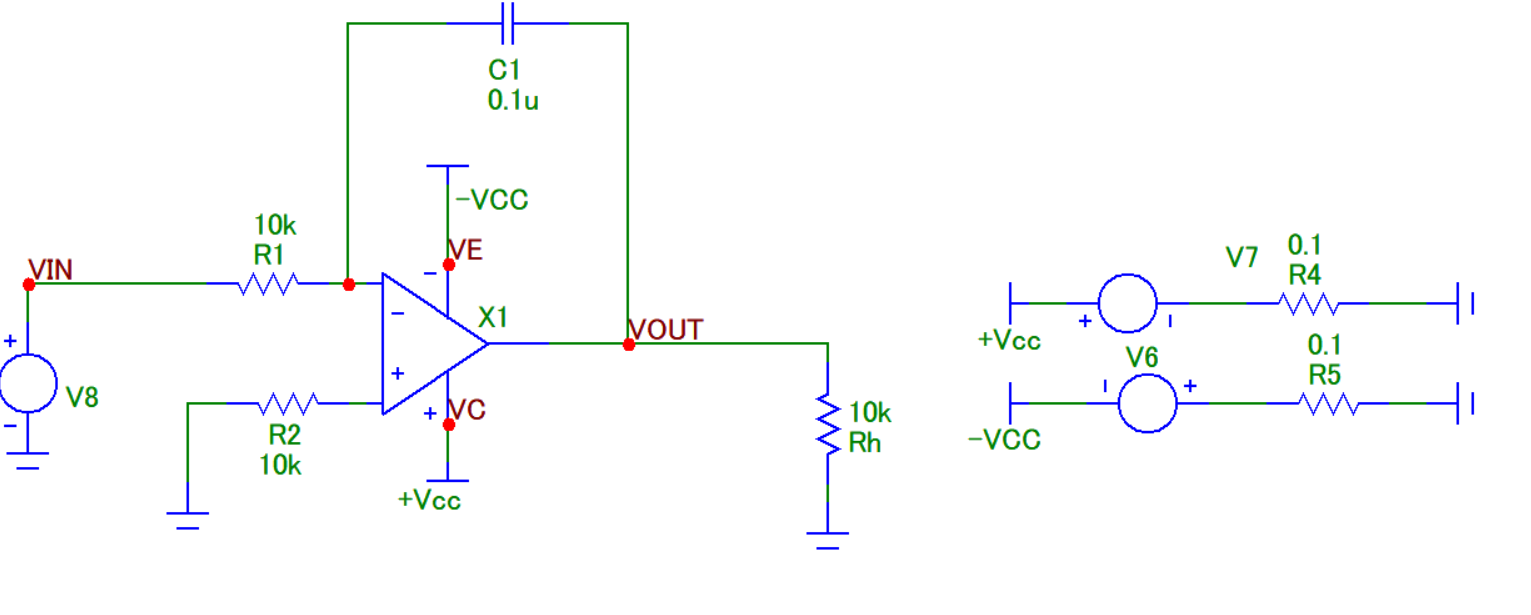
\includegraphics[width=\linewidth]{../imgs/schema_int_base}
	\caption{Схема инвертирующего интегратора}
	\label{fig:schema_int_base}
\end{figure}

\begin{figure}[H]
	\centering
	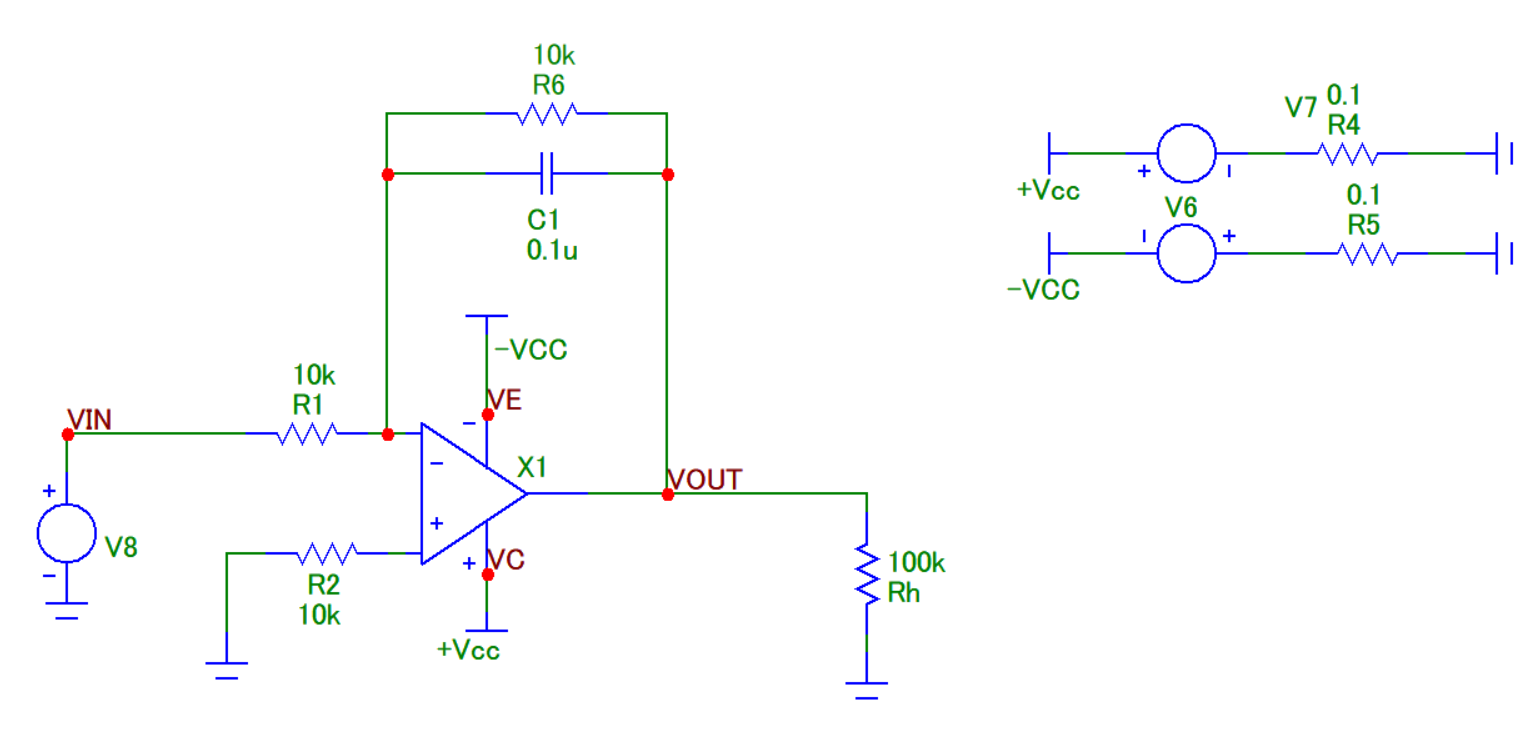
\includegraphics[width=\linewidth]{../imgs/schema_int}
	\caption{Схема инвертирующего интегратора с шунтирующим сопротивлением}
	\label{fig:schema_int}
\end{figure}

\subsection{Исследование выходных сигналов на различных частотах}

\subsubsection{Гармонический сигнал}

\begin{figure}[H]
	\centering
	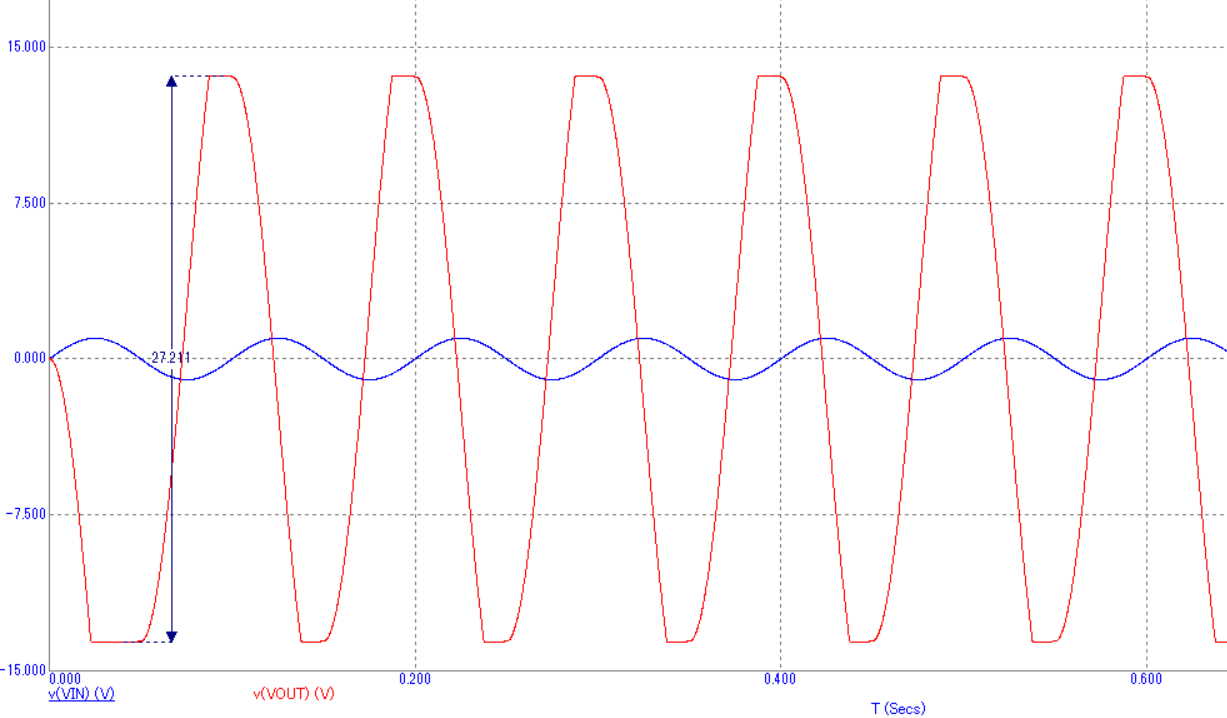
\includegraphics[width=0.9\linewidth]{../imgs/tran_sin_10Hz}
	\caption{Осциллограмма для гармонического сигнала при частоте 10 Гц}
	\label{fig:tran_sin_10Hz}
\end{figure}

Амплитуда выходного сигнала $27.2V$ (рис. \ref{fig:tran_sin_10Hz})

\begin{figure}[H]
	\centering
	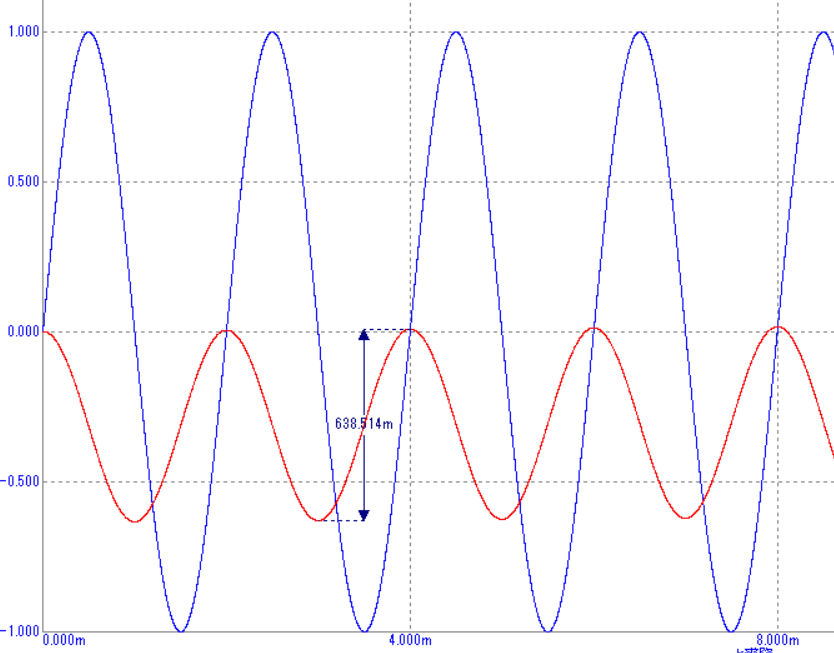
\includegraphics[width=0.7\linewidth]{../imgs/tran_sin_500Hz}
	\caption{Осциллограмма для гармонического сигнала при частоте 500 Гц}
	\label{fig:tran_sin_500Hz}
\end{figure}

Амплитуда выходного сигнала $0.639V$ (рис. \ref{fig:tran_sin_500Hz})

\subsubsection{Квадратичный сигнал}

\begin{figure}[H]
	\centering
	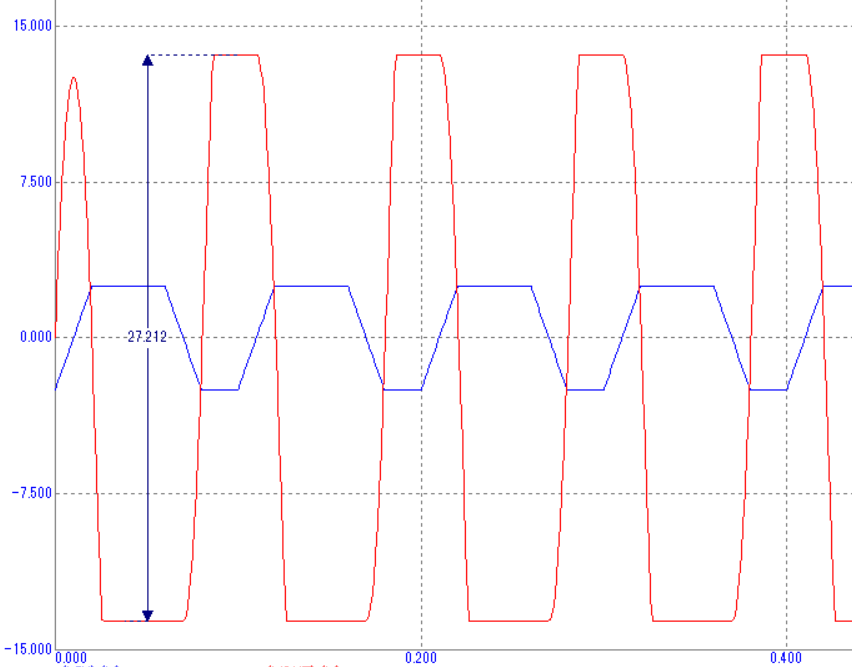
\includegraphics[width=0.7\linewidth]{../imgs/tran_square_10Hz}
	\caption{Осциллограмма для квадратичного сигнала при частоте 10 Гц}
	\label{fig:tran_square_10Hz}
\end{figure}

Амплитуда выходного сигнала $27.2V$ (рис. \ref{fig:tran_square_10Hz})

\begin{figure}[H]
	\centering
	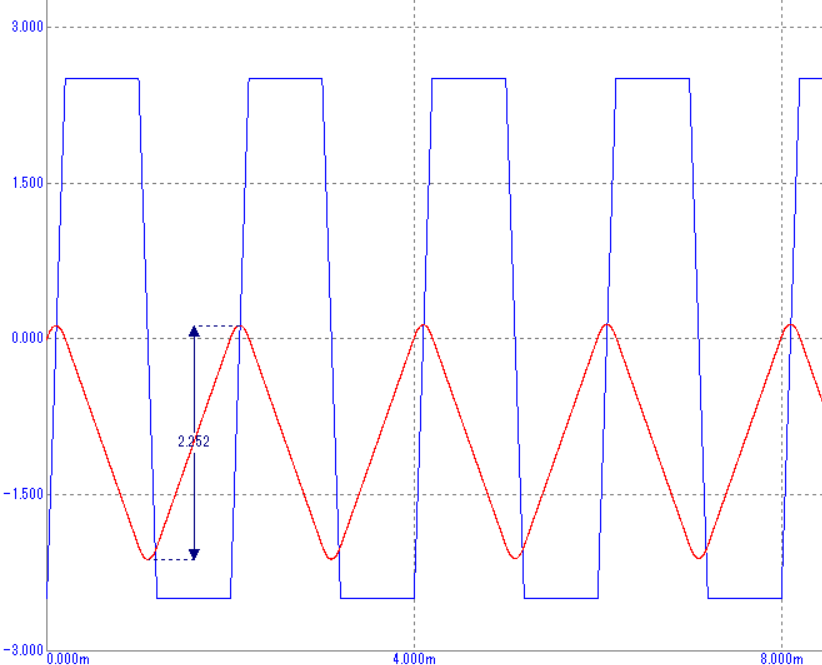
\includegraphics[width=0.7\linewidth]{../imgs/tran_square_500Hz}
	\caption{Осциллограмма для квадратичного сигнала при частоте 500 Гц}
	\label{fig:tran_square_500Hz}
\end{figure}

Амплитуда выходного сигнала $2.25V$ (рис. \ref{fig:tran_square_500Hz})

\subsubsection{Треугольный сигнал}

\begin{figure}[H]
	\centering
	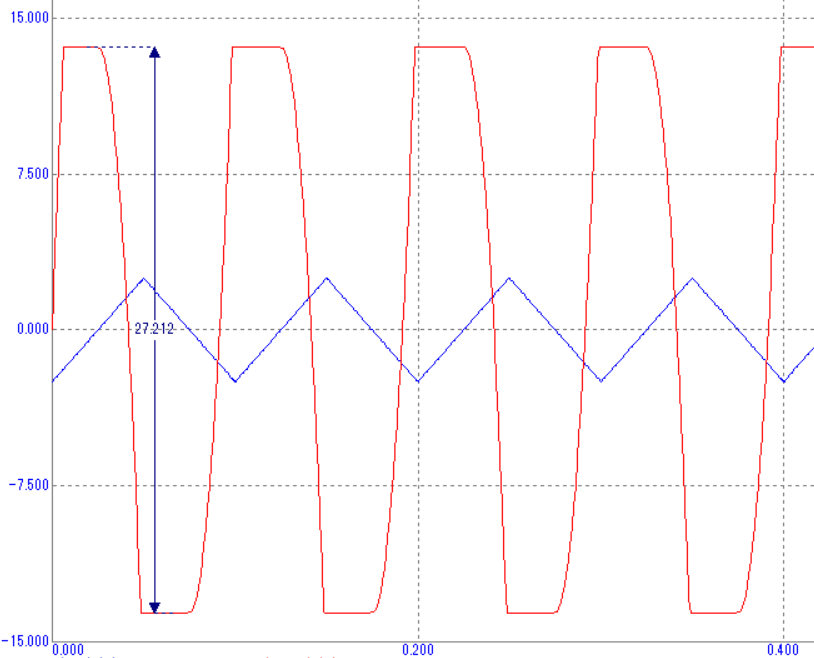
\includegraphics[width=0.7\linewidth]{../imgs/tran_triangle_10Hz}
	\caption{Осциллограмма для треугольного сигнала при частоте 10 Гц}
	\label{fig:tran_triangle_10Hz}
\end{figure}

Амплитуда выходного сигнала $27.5V$ (рис. \ref{fig:tran_triangle_10Hz})

\begin{figure}[H]
	\centering
	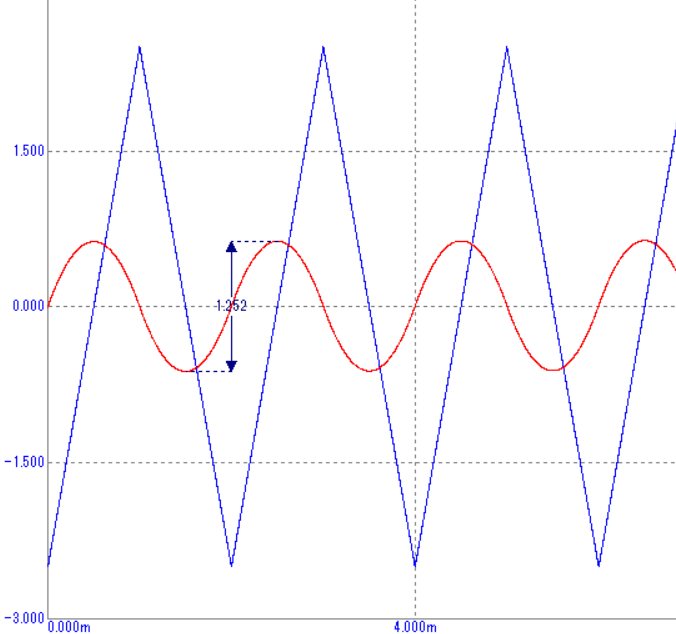
\includegraphics[width=0.7\linewidth]{../imgs/tran_triangle_500Hz}
	\caption{Осциллограмма для треугольного сигнала при частоте 500 Гц}
	\label{fig:tran_triangle_500Hz}
\end{figure}

Амплитуда выходного сигнала $1.25V$ (рис. \ref{fig:tran_triangle_500Hz})

\subsection{Исследование АЧХ и ФЧХ интегратора}

\begin{figure}[H]
	\centering
	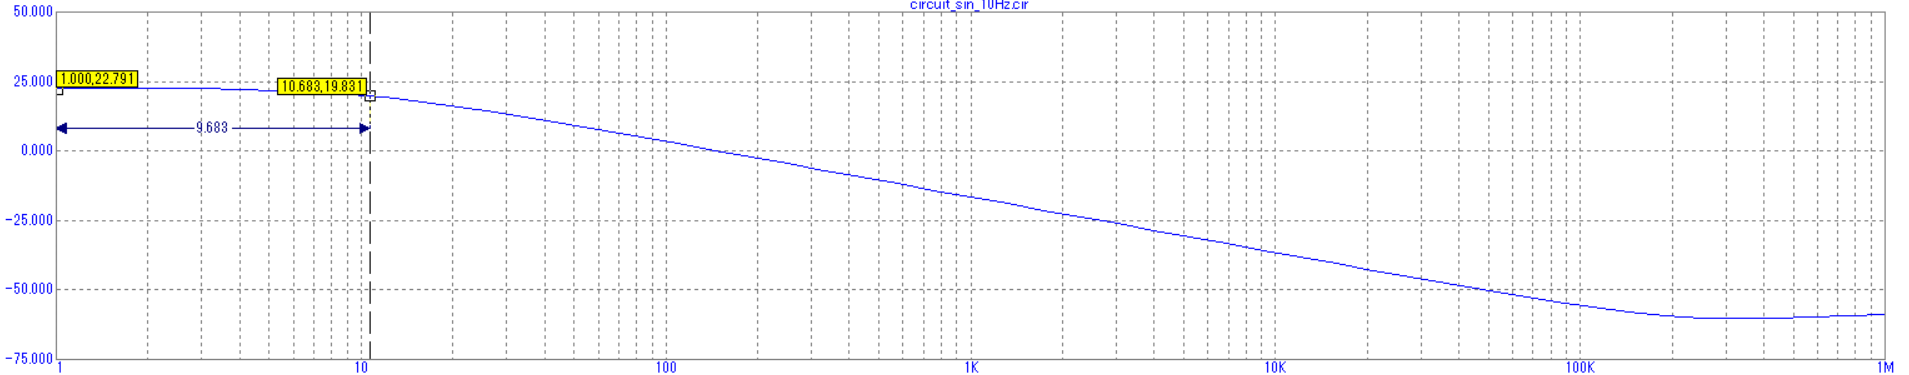
\includegraphics[width=\linewidth]{../imgs/int_fr}
	\caption{АЧХ интегратора}
	\label{fig:int_fr}
\end{figure}


Частота среза: $10.6Hz$

Полоса пропускания: $1Hz - 10.6Hz$

\begin{figure}[H]
	\centering
	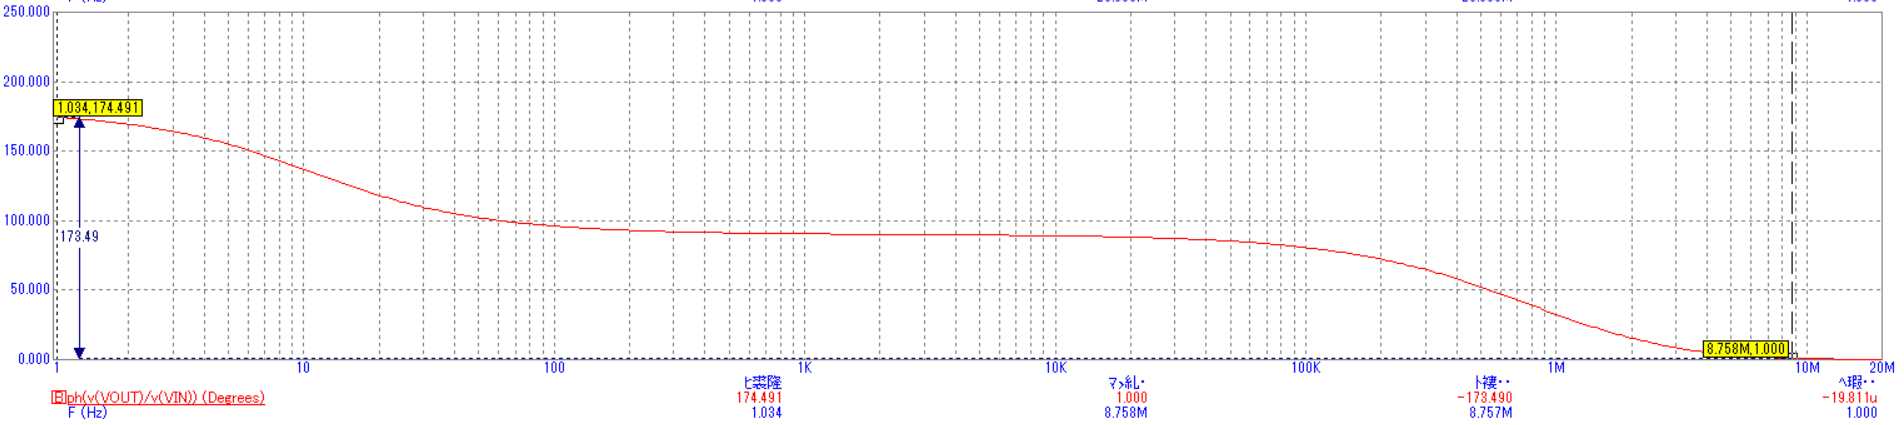
\includegraphics[width=\linewidth]{../imgs/int_pr}
	\caption{ФЧХ интегратора}
	\label{fig:int_pr}
\end{figure}

Максимальный фазовый сдвиг: $173.5^{\circ}$

Наклон ФЧХ: $-19.811$

\section{Инвертирующий дифференциатор}

В программе Micro-Cap была создана схема инвертирующего дифференциатора с увеличенной устойчивостью к возбуждению(рис. \ref{fig:schema_diff}).

\begin{figure}[H]
	\centering
	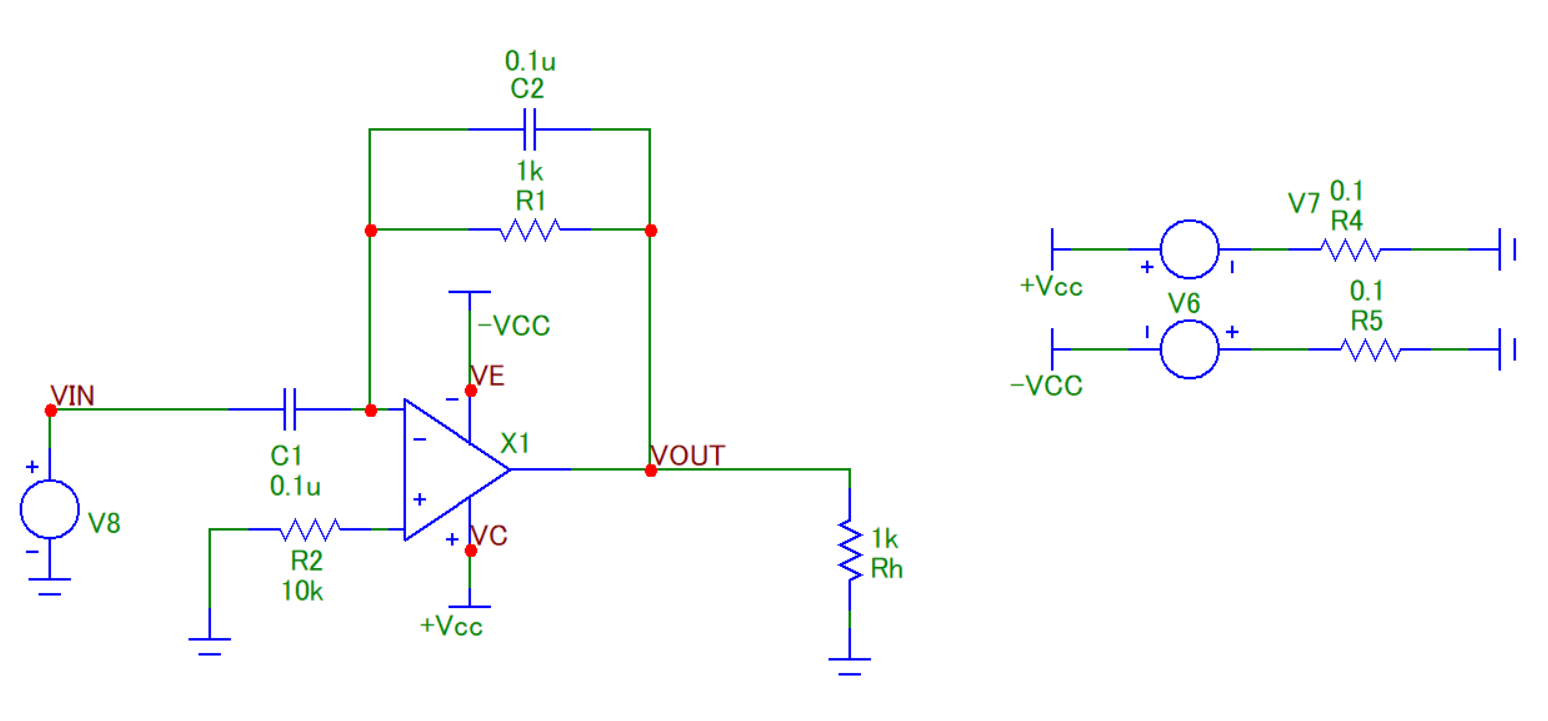
\includegraphics[width=\linewidth]{../imgs/schema_diff}
	\caption{Схема инвертирующего дифференциатора}
	\label{fig:schema_diff}
\end{figure}

\subsection{Исследование выходных сигналов на различных частотах}

\subsubsection{Гармонический сигнал}

\begin{figure}[H]
	\centering
	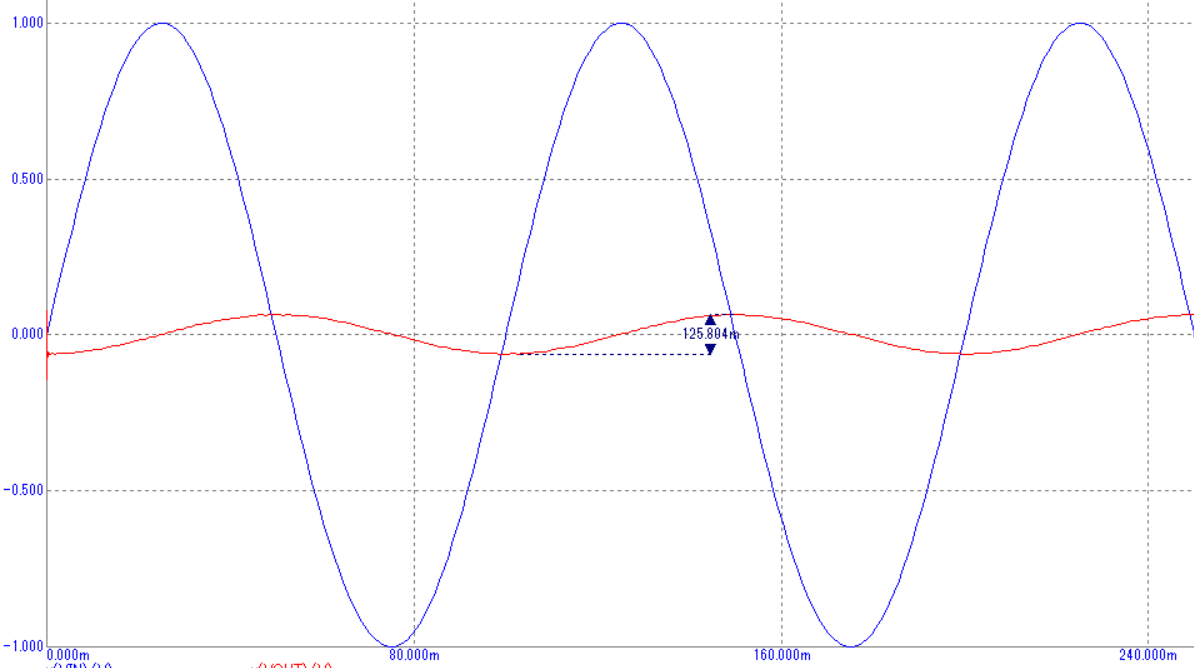
\includegraphics[width=0.9\linewidth]{../imgs/tran_sin_10Hz_diff}
	\caption{Осциллограмма для гармонического сигнала при частоте 10 Гц}
	\label{fig:tran_sin_10Hz_diff}
\end{figure}

Амплитуда выходного сигнала $0.125V$ (рис. \ref{fig:tran_sin_10Hz_diff})

\begin{figure}[H]
	\centering
	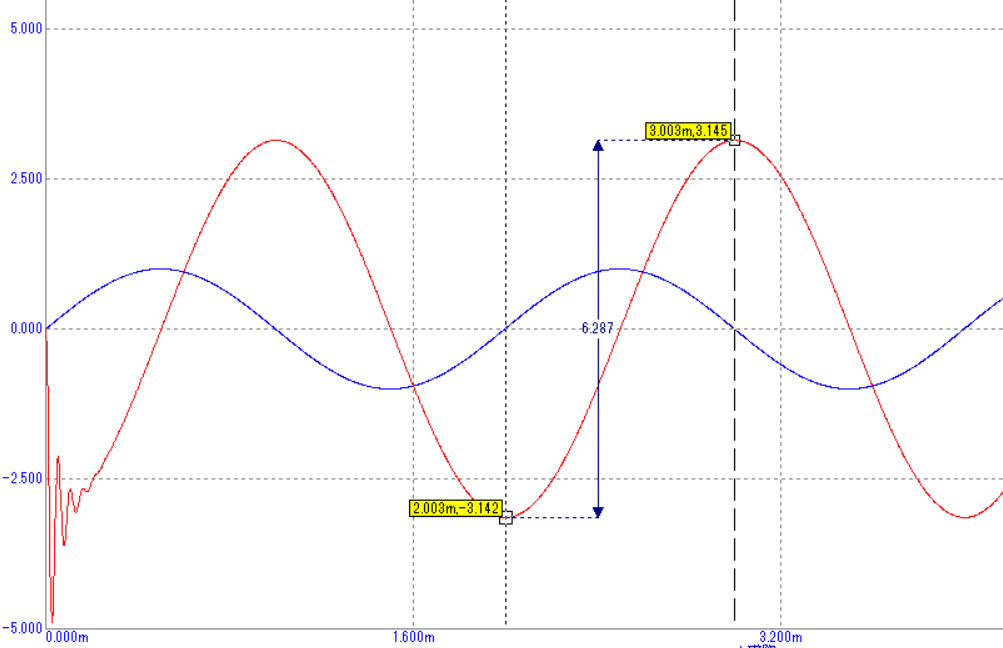
\includegraphics[width=0.7\linewidth]{../imgs/tran_sin_500Hz_diff}
	\caption{Осциллограмма для гармонического сигнала при частоте 500 Гц}
	\label{fig:tran_sin_500Hz_diff}
\end{figure}

Амплитуда выходного сигнала $6.29V$ (рис. \ref{fig:tran_sin_500Hz_diff})

\subsubsection{Квадратичный сигнал}

\begin{figure}[H]
	\centering
	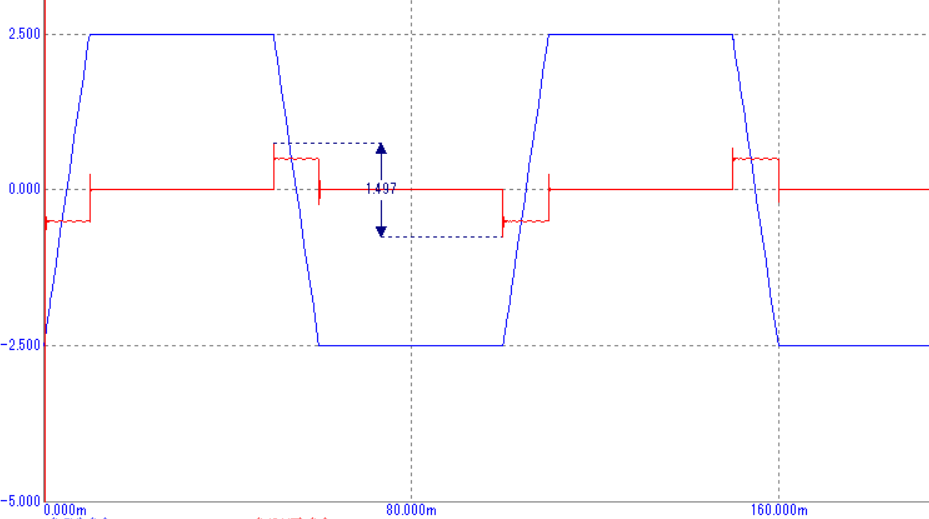
\includegraphics[width=0.7\linewidth]{../imgs/tran_square_10Hz_diff}
	\caption{Осциллограмма для квадратичного сигнала при частоте 10 Гц}
	\label{fig:tran_square_10Hz_diff}
\end{figure}

Амплитуда выходного сигнала $1.50V$ (рис. \ref{fig:tran_square_10Hz_diff})

\begin{figure}[H]
	\centering
	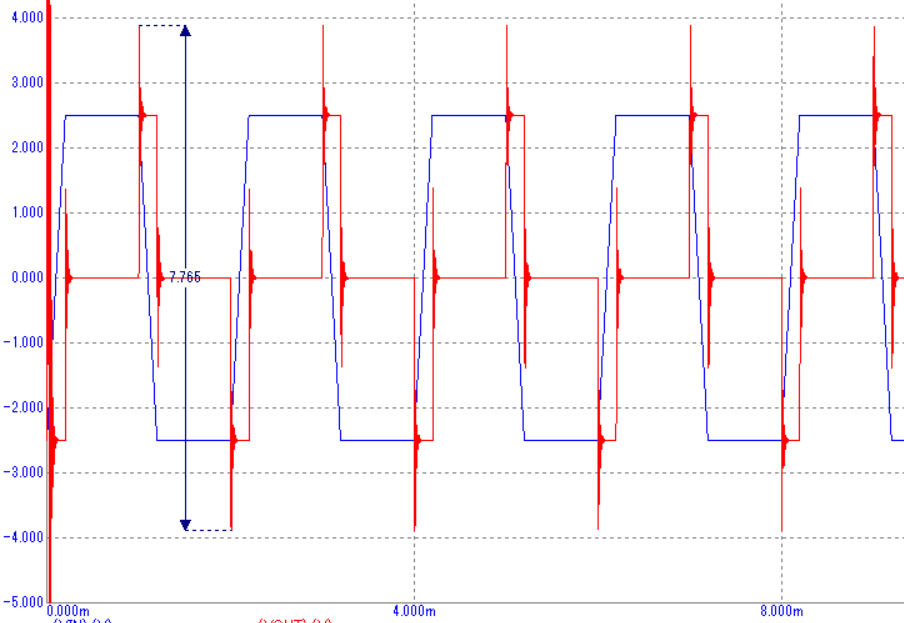
\includegraphics[width=0.7\linewidth]{../imgs/tran_square_500Hz_diff}
	\caption{Осциллограмма для квадратичного сигнала при частоте 500 Гц, $С_2=1nF R_1 = 1kOhm$}
	\label{fig:tran_square_500Hz_diff}
\end{figure}

Амплитуда выходного сигнала $7.77V$ (рис. \ref{fig:tran_square_500Hz_diff})

\subsubsection{Треугольный сигнал}

\begin{figure}[H]
	\centering
	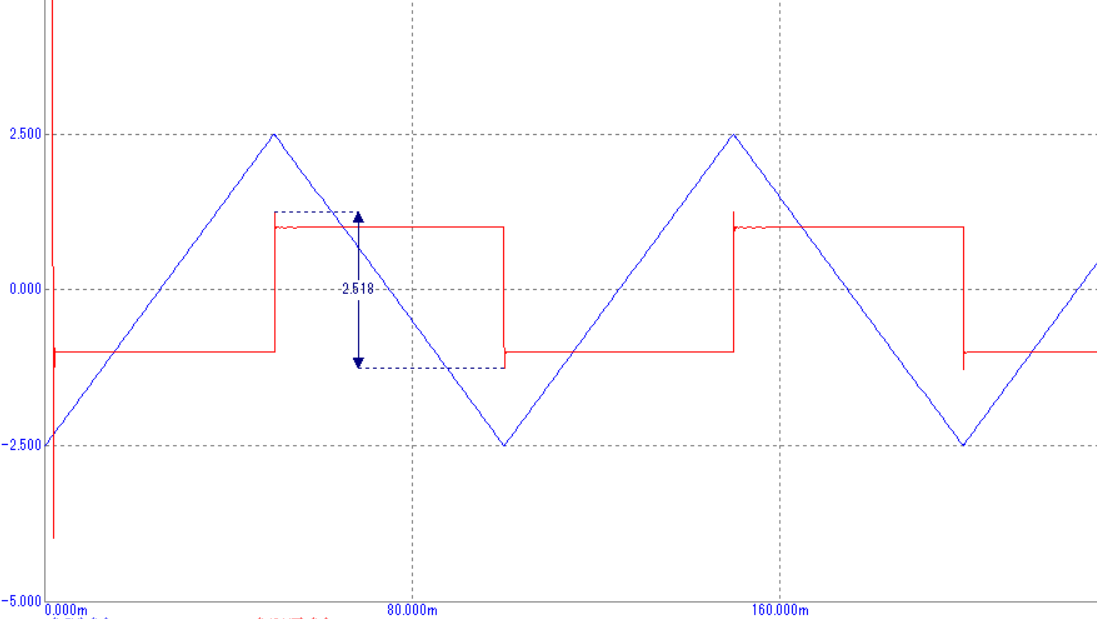
\includegraphics[width=0.7\linewidth]{../imgs/tran_triangle_10Hz_diff}
	\caption{Осциллограмма для треугольного сигнала при частоте 10 Гц, $R_1 = 100kOhm$}
	\label{fig:tran_triangle_10Hz_diff}
\end{figure}

Амплитуда выходного сигнала $2.52V$ (рис. \ref{fig:tran_triangle_10Hz_diff})

\begin{figure}[H]
	\centering
	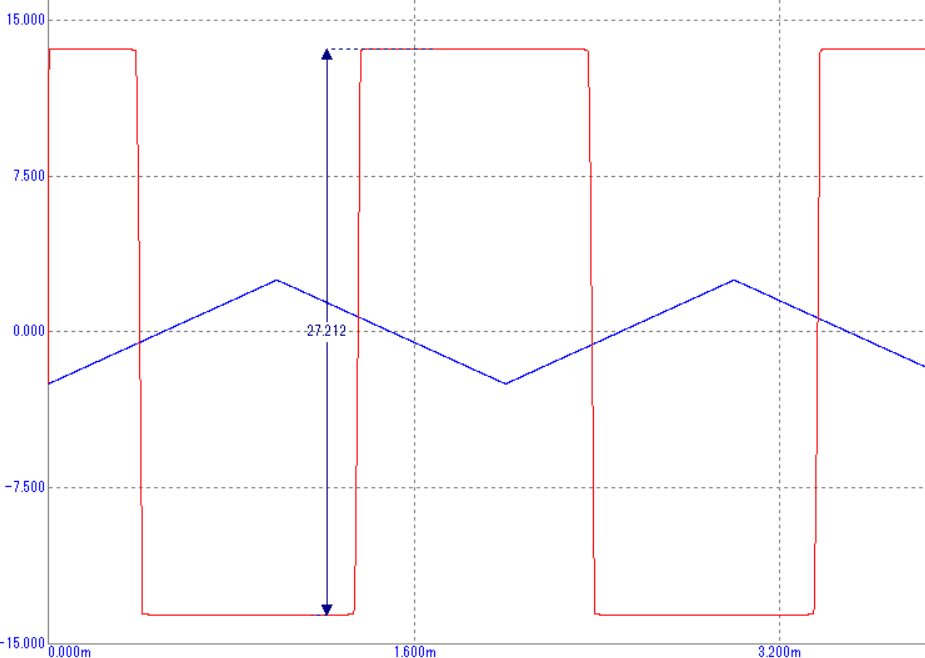
\includegraphics[width=0.7\linewidth]{../imgs/tran_triangle_500Hz_diff}
	\caption{Осциллограмма для треугольного сигнала при частоте 500 Гц, $R_1 = 1kOhm$}
	\label{fig:tran_triangle_500Hz_diff}
\end{figure}

Амплитуда выходного сигнала $27.2V$ (рис. \ref{fig:tran_triangle_500Hz_diff})

\subsection{Исследование АЧХ и ФЧХ дифференциатора}

\begin{figure}[H]
	\centering
	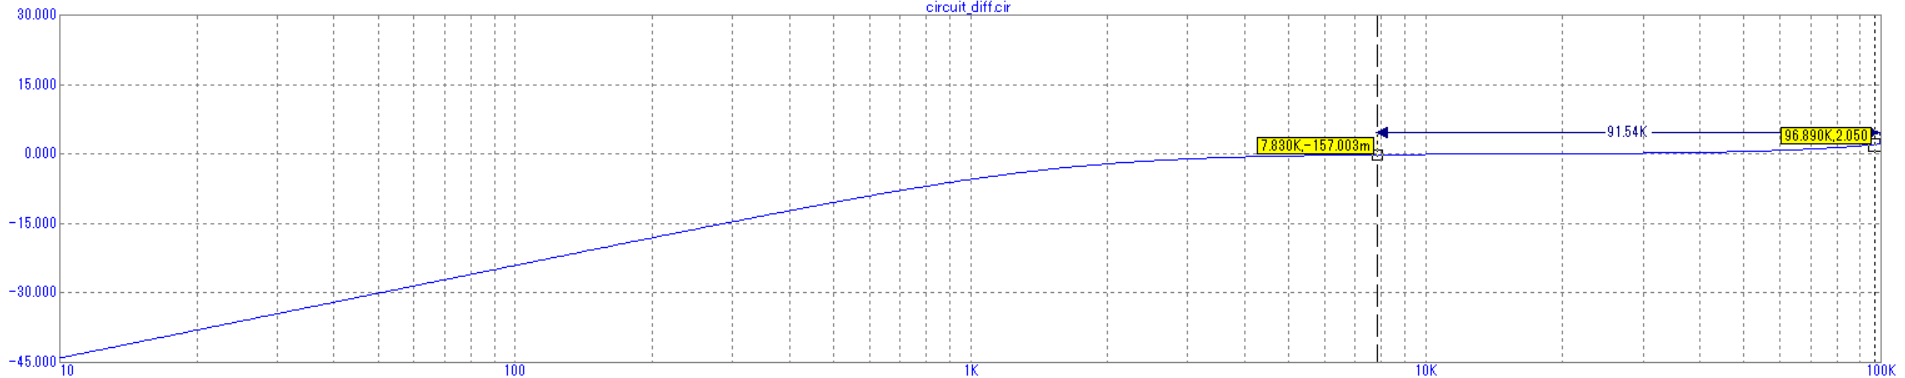
\includegraphics[width=\linewidth]{../imgs/diff_fr}
	\caption{АЧХ дифференциатора}
	\label{fig:diff_fr}
\end{figure}

Частота среза: $7830Hz$

Полоса пропускания: $7.83kHz - 100kHz$

Ширина полосы пропускания: $92.17kHz$

\begin{figure}[H]
	\centering
	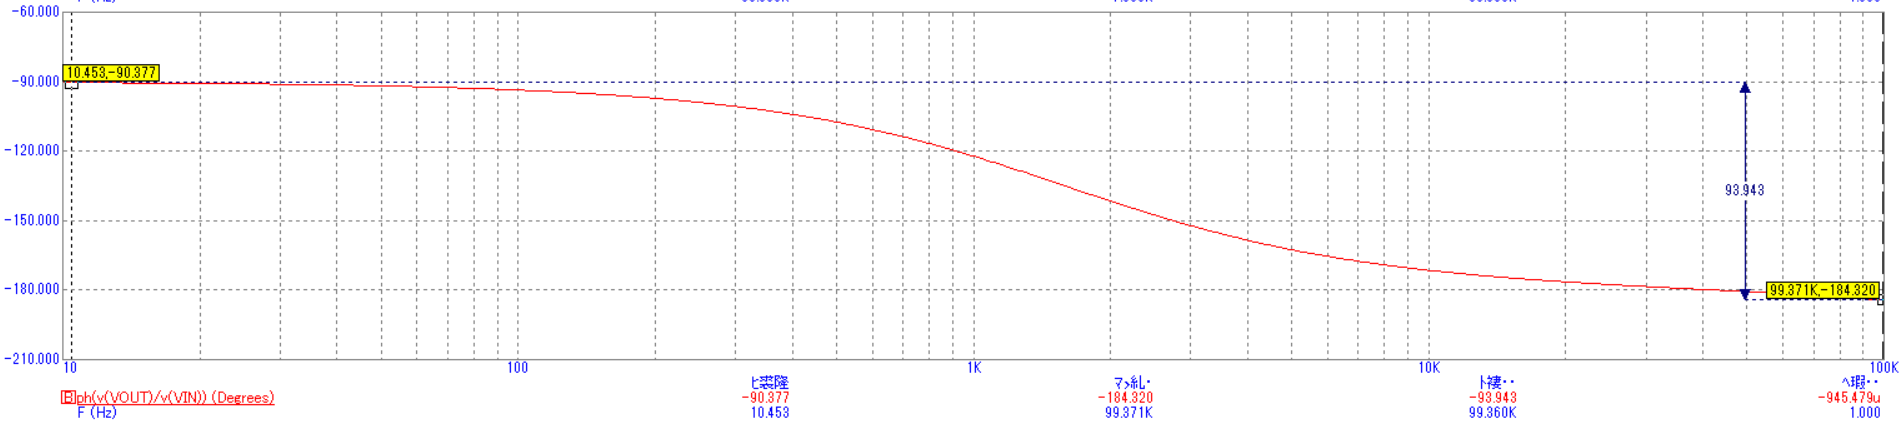
\includegraphics[width=\linewidth]{../imgs/diff_pr}
	\caption{ФЧХ дифференциатора}
	\label{fig:diff_pr}
\end{figure}

Максимальный фазовый сдвиг: $93.9^{\circ}$

Наклон ФЧХ: $-0.945$

\end{document} % конец документа






